\documentclass[a4paper,12pt]{article}
\usepackage{geometry}
\usepackage{hyperref}
\usepackage{booktabs}
\usepackage{array}
\usepackage{longtable}
\usepackage{caption}
\usepackage{graphicx}
\usepackage{multirow}
\usepackage{multicol}

\geometry{margin=1in}
\hypersetup{
    colorlinks=true,
    linkcolor=blue,
    urlcolor=blue
}

\title{Nova-CAN Communication Standard}
\author{Taaj Street, Matt van Wijk, Anthony Verbini, Harrison Ryan}
\date{May, 2025}

\begin{document}

\maketitle
\tableofcontents
\newpage

\section{Introduction}
This specification is heavily inspired by the \href{https://opencyphal.org/}{OpenCyphal} protocol \href{https://opencyphal.org/specification/Cyphal_Specification.pdf}{specification}, specifically Cyphal/CAN. There are changes to make the protocol simpler and more applicable to NovaRover's use case.

\section{Communication Model}
Nova-CAN will be based primarily on:
\begin{itemize}
    \item \textbf{One-to-one messages} (one-way)
    \item \textbf{Services} (two-way)
\end{itemize}

Additionally, one-to-many communication is available in specific scenarios (e.g., system-wide halt messages and telemetry from devices). This differs from the OpenCyphal protocol where only services contain both destination and source node IDs. The modification was made due to the resource-constrained microcontrollers used in NovaRover devices, which require hardware-level CAN filtering to reduce load.

\subsection{Definitions}
\begin{description}
    \item[Node:] Each device is a node with a unique 6-bit device ID. Valid values are \([1{-}127]\).
    \item[Message:] A one-way, one-to-one or one-to-many communication.
    \item[Service:] A two-way, one-to-one request/response communication.
    \item[Subject:] Messages and services are sent/received/invoked on subjects. A subject is a 9-bit identifier, allowing:
    \begin{itemize}
        \item 512 send subjects
        \item 512 receive subjects
    \end{itemize}
    Each subject is of a predefined data type (see Section~\ref{sec:msg-layout}). Protocol Subjects (defined in Section~\ref{sec:protocol-subjects}) must be implemented by all nodes. Each node also has:
    \begin{itemize}
        \item Subscribed subjects
        \item Published subjects
        \item Parameter subjects
    \end{itemize}
    These are defined by device interfaces (see \textit{Device Interface} section).
\end{description}
\newpage

\section{CAN-ID Layout}
The bit layout for a CAN-ID is shown in Figure~\ref{fig:canid-layout}.

\begin{figure}[h!]
    \centering
    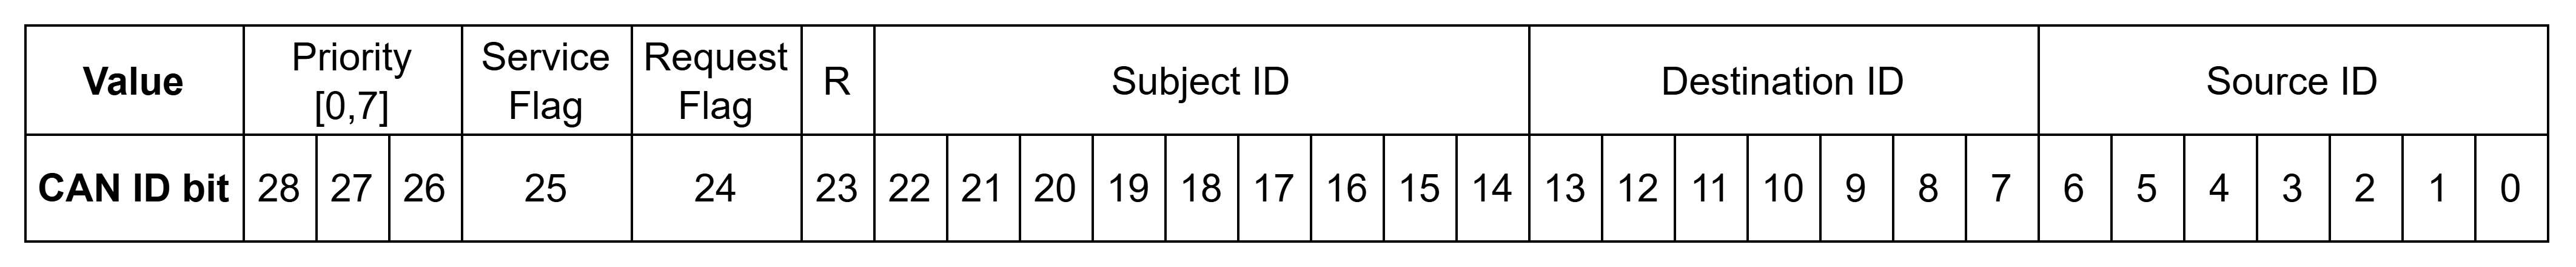
\includegraphics[width=1.0\linewidth]{figures/CANID_bitlayout.png}
    \caption{CAN-ID Bit Layout}
    \label{fig:canid-layout}
\end{figure}

\begin{longtable}{@{}p{3cm}p{2cm}p{5cm}p{5cm}@{}}
\toprule
\textbf{Field}       & \textbf{Width (bits)} & \textbf{Valid Values}                & \textbf{Description} \\ \midrule
Priority             & 3                     & \([0{-}7]\)                         & Message priority from 0–7 (see \textit{Priority}). \\ \midrule
Service Flag         & 1                     & \([0,1]\)                           & 0 for message, 1 for service. \\ \midrule
Request Flag         & 1                     & 0 for messages \newline \([0,1]\) for services & 
If service flag is 0, request flag must also be 0 (frame discarded otherwise). \newline
If service flag is 1, request flag = 1 for service request, 0 for service response. \\ \midrule
R (Reserved)         & 1                     & 0                                   & Reserved for future use. \\ \midrule
Subject ID           & 9                     & \([0{-}511]\)                       & Represents a specific data type (see \textit{DSDL section}). \newline Per-node, allowing up to 512 subjects (messages/services). \\ \midrule
Destination ID       & 6                     & 0 reserved for multicast. \newline \([1{-}127]\) for node-specific messages/services & 
Destination node ID. \newline
0 = multicast message (multicast services are invalid). \newline
Frames with destination ID 0 and service flag 1 are invalid. \\ \midrule
Source ID            & 6                     & \([1{-}127]\)                       & Source node ID (0 is invalid). \\ \bottomrule
\end{longtable}
\newpage
\section{Message Data Layout and Encoding}
\label{sec:msg-layout}
\subsection{Frame Header}
All frames shall have a one-byte header as seen in Table \ref{tab:header-byte-structure}
\begin{table}[h]
\centering
\caption{Header Byte Structure}
\label{tab:header-byte-structure}
\renewcommand{\arraystretch}{1.3} % spacing between rows
\begin{tabular}[h]{|c|l|l|l|}
\hline
\textbf{Bit} & \textbf{Field} & \textbf{Single-frame transfers} & \textbf{Multi-frame transfers} \\
\hline
7 & \textbf{Start of transfer} & Always 1 & First frame: 1, otherwise 0. \\
\hline
6 & \textbf{End of transfer} & Always 1 & Last frame: 1, otherwise 0. \\
\hline
5 & \textbf{Toggle bit} & Always 1 & First frame: 1, then alternates; \\
\hline
4 & \multirow{3}{*}{\textbf{Transfer-ID}} & \multicolumn{2}{c|}{\multirow{3}{*}{\centering Modulo 32 (range [0, 31])}} \\
\cline{1-1}
3 & & \multicolumn{2}{c|}{} \\
\cline{1-1}
2 & & \multicolumn{2}{c|}{} \\
\cline{1-1}
1 &  & \multicolumn{2}{c|}{} \\
\cline{1-1}
0 &  & \multicolumn{2}{c|}{} \\
\hline
\end{tabular}
\end{table}

\begin{description}
    \item[Start of transfer]: Flag for the start of a transfer. This allows detecting the start of a multi-frame message.
    \item[End of transfer]: Flag for the end of a transfer. This allows detecting the end of a multi-frame message.
    \item[Toggle bit]: Toggles on alternate frames of multi-bit messages. Used for deduplication of messages.
    \item[Transfer-ID:] Cyclic modulo 32 transfer ID for the subject. Increments for every transfer. This is used for multiframe reconstruction and service call matching to allow multiple service calls from the same client to server. Transfer ID for a service response is not incremented, it is copied.
\end{description}

\subsection{CRC}
Multi-frame transfers require a CRC to check data-integrity across the entire message. This shall be added to the final frame of the message.
\textit{(TODO: define the exact CRC used)}

\subsection{Data Definition and Format}
All messages shall be defined through a message description language. Version 0 of this specification will rely upon the \textit{OpenCyphal Data Structure Description Language}, described \href{https://opencyphal.org/specification/Cyphal_Specification.pdf#page=15}{here} in it's specification, and the open-source \href{https://github.com/OpenCyphal/nunavut}{nunavut} transpiler to generate C, C++ and Python3 types.
\section{Protocol Subjects}
\label{sec:protocol-subjects}
\textit{(To be completed)}

\section{Device Interface}
\label{sec:device-interface}
\textit{(To be completed)}

\section{System Description}
\label{sec:system-description}
\textit{(To be completed)}

\end{document}